\documentclass[10pt,border=0pt]{standalone}

\usepackage[utf8]{inputenc}
\usepackage{amssymb,amsmath}
\usepackage{tikz}



\thispagestyle{empty}

\begin{document}

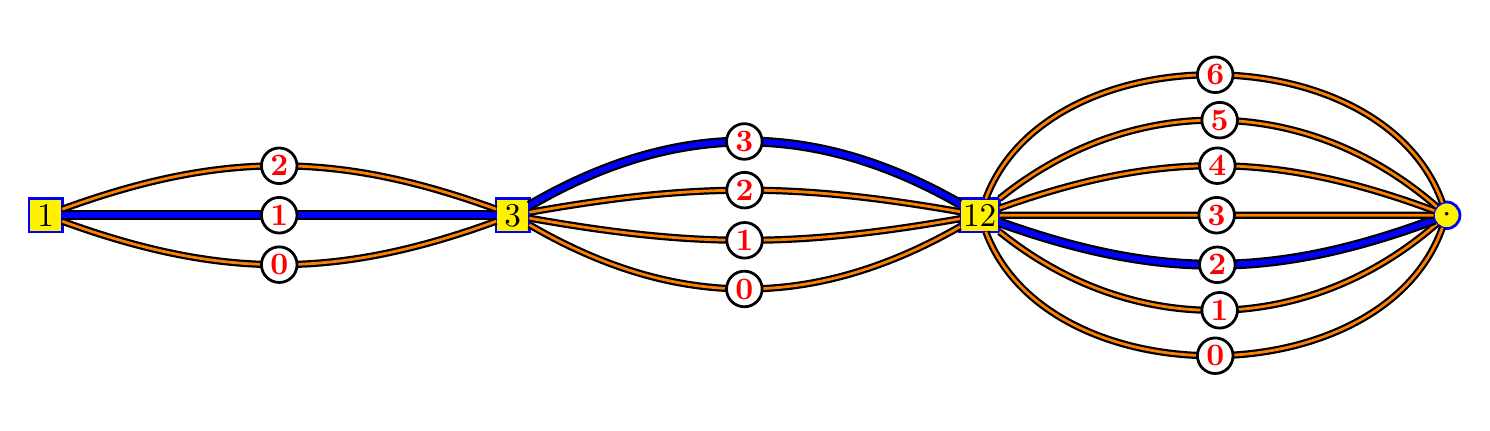
\begin{tikzpicture}[x=9pt,y=6pt,scale=1.5, transform shape]
  \centering
  \tikzset{VertexStyle/.style = {
    shape         = rectangle,
    draw          = blue,
    fill          = yellow,
  	line width    = 1pt,
    text          = black,
    inner sep     = 1pt,
    outer sep     = 0pt,
    minimum size  = 10 pt,
    scale         = 0.8
    }
  }
  \tikzset{VertexStyle2/.style = {
    shape         = circle,
    draw          = blue,
    fill          = yellow,
  	line width    = 1pt,
    text          = black,
    inner sep     = 1pt,
    outer sep     = 0pt,
    minimum size  = 5 pt,
    scale         = 0.8
    }
  }
  \tikzset{EdgeStyle/.style = {
    draw            = black,
    thick,
    double          = orange,
    double distance = 1pt
    }
  }
  \tikzset{EdgeStylePath/.style = {
    draw            = black,
    thick,
    double          = blue,
    double distance = 2pt
    }
  }
  \tikzset{EdgeLabelStyle/.style = {
    draw          = black,
  	shape         = circle,
  	line width    = 1pt,
  	minimum size  = 10pt,
    inner sep     = 1pt,
    outer sep     = 0pt,
    fill          = white,
    text          = red,
    scale         = 0.75
    }
  }

	\node[VertexStyle](A1) at (6.25, 25) {$1$};
	\node[VertexStyle](B1) at (18.75, 25) {$3$};
	\node[VertexStyle](C1) at (31.25, 25) {$12$};
	\node[VertexStyle2](D1) at (43.75, 25) {$\cdot$};
	\draw[EdgeStyle, bend left=-20](A1) to node[EdgeLabelStyle]{$\bf 0$} (B1);
	\draw[EdgeStylePath, bend left=0](A1) to node[EdgeLabelStyle]{$\bf 1$} (B1);
	\draw[EdgeStyle, bend left=20](A1) to node[EdgeLabelStyle]{$\bf 2$} (B1);
	\draw[EdgeStyle, bend left=-30](B1) to node[EdgeLabelStyle]{$\bf 0$} (C1);
	\draw[EdgeStyle, bend left=-10](B1) to node[EdgeLabelStyle]{$\bf 1$} (C1);
	\draw[EdgeStyle, bend left=10](B1) to node[EdgeLabelStyle]{$\bf 2$} (C1);
	\draw[EdgeStylePath, bend left=30](B1) to node[EdgeLabelStyle]{$\bf 3$} (C1);
	\draw[EdgeStyle, bend left=-70](C1) to node[EdgeLabelStyle]{$\bf 0$} (D1);
	\draw[EdgeStyle, bend left=-40](C1) to node[EdgeLabelStyle]{$\bf 1$} (D1);
	\draw[EdgeStylePath, bend left=-20](C1) to node[EdgeLabelStyle]{$\bf 2$} (D1);
	\draw[EdgeStyle, bend left=0](C1) to node[EdgeLabelStyle]{$\bf 3$} (D1);
	\draw[EdgeStyle, bend left=20](C1) to node[EdgeLabelStyle]{$\bf 4$} (D1);
	\draw[EdgeStyle, bend left=40](C1) to node[EdgeLabelStyle]{$\bf 5$} (D1);
	\draw[EdgeStyle, bend left=70](C1) to node[EdgeLabelStyle]{$\bf 6$} (D1);

  \end{tikzpicture}

\end{document}
